\section{安全性分析}
本章提出的隐私保护神经网络的线性计算部分采用秘密分享进行设计,在半可信安全性设定下满足信息论安全~\cite{demmler2015aby}。
%
因此,本节讨论基于随机排列的非线性激活函数计算的安全性。
%
尽管前文已经展示了可能的随机排列个数随着元素个数$n$的增长而超指数增长,本节采用了更加精确的量化手段基于分析。
%
具体而言,本节采用了距离相关性(Distance Correlation)作为安全性指标,对于随机排列以及简单的线性变换(拆分学习中直接暴露中间结果的情况)进行了分析,显示了随机排列带来的隐私泄露极小。

\subsection{距离相关性}
距离相关性(Distance Correlation)~\cite{szekely2007dcor,szekely2009brownian_dcor}是一种统计学上的相关性度量,可以度量任意两个高维向量之间的相关性。
相对于常用的皮尔逊相关性系数,距离相关性可以对任意两个不同维度的高维随机向量进行建模,并且可以捕获非线性的相关性,只有在两个随机向量完全无关时才会为0。
%
\begin{definition}[距离相关性]
    对于两个随机向量$X \in \mathbb R^p, Y\in \mathbb R^q$,距离相关性的定义为
    \begin{equation}
        \textnormal{DCOR}(X, Y) = \dfrac{\mathcal{V}(X, Y)^2}{\sqrt{\mathcal{V}(X, X)^2\mathcal{V}(Y, Y)^2}},
    \end{equation}
    其中$\mathcal{V}$表示距离协方差(Distance Covariance),定义如下
    \begin{equation}
        \mathcal{V}(X, Y)^2 = \dfrac{1}{c_pc_q} \int_{\mathbb R^{p + q}}
        \dfrac{|f_{X, Y}(t, s) - f_X(t)f_Y(s)|^2}{\Vert c_p \Vert^{p+1}\Vert c_q \Vert^{q+1}}dtds,
    \end{equation}
    其中,$c_p, c_q$为两个常数,$\Vert \cdot \Vert$表示欧几里得范数(Euclidean Norm)。
\end{definition}

除去上述的定义为,距离协方差还可以通过
\begin{equation}
\begin{split}
    \mathcal{V}(X, Y)^2 = 
    & \quad \mathbb E \Vert X-X'\Vert \Vert Y -Y'\Vert +\mathbb E\Vert X -X' \Vert \mathbb E \Vert Y -Y' \Vert
    \\ & 
    - \mathbb E\Vert X-X'\Vert  \Vert Y -Y''\Vert - \mathbb E \Vert X -X''\Vert  \Vert Y -Y' \Vert
\end{split}
\end{equation}
来计算,其中$(X, Y), (X', Y'), (X'', Y'')$是相互独立的。
%
通过上式可以以采样的方式来估算距离相关性。

\subsection{随机线性变换的距离相关性}
现在我们研究随机线性变换后的向量与随机变换之前的向量的距离相关性。
我们用$\angle[\cdot, \cdot]$表示两个向量之间的夹角。
\begin{theorem}
\label{thm:ss-perm:linear-dcov}
    令$X\in \mathbb R^n$是一个随机的$n$维随机向量,令$Y = AX$,
    %
    其中 $A \in \mathbb R^{n \times d}$是一个随机线性变换,并且满足在单位正交变换下概率不变,即$P(A) = P(AT)$, $T$是$n$维单位正交矩阵(Orthonormal Matrix)。
    %
    则
    \begin{equation}
    \label{eq:ss-perm:linear-dcov1}
            \mathop{\mathbb E}_A \mathcal{V}(X, AX)^2 = a\mathcal{V}(X, X)^2,
    \end{equation}
    以及    
    \begin{equation}
    \label{eq:ss-perm:linear-dcov2}
        \mathop{\mathbb E}_A \mathcal{V}(AX, AX)^2 = {a^2S_1 + b^2S_2 - 2S_3'},
    \end{equation}
    其中 $S_1 = \mathbb \Vert X - X'\Vert^2, S_2 = \left( \mathbb E \Vert X - X'\Vert \right)^2, S_3 = \mathbb E \Vert X - X' \Vert \Vert X - X'' \Vert$,\\
    $S' = \mathbb E \left[ g(\angle [X - X', X - X'']) \cdot \Vert X - X'\Vert \Vert X - X'' \Vert \right]$,
    以及
    $g_A(\theta) = \mathbb E_A \dfrac{\Vert A\bvec x \Vert \Vert A\bvec y \Vert}{\Vert \bvec x \Vert \Vert \bvec y \Vert} $,
    $a = \mathbb E_A \dfrac{\Vert A\bvec x \Vert}{\Vert \bvec x \Vert}$,
    $b = \sqrt{\mathbb E_A \dfrac{\Vert A\bvec x \Vert^2}{\Vert \bvec x \Vert^2}}$,$\bvec x, \bvec y$为任意的$n$维向量,且夹角为$\theta$。
\end{theorem}
\begin{proof}
我们用$\mathbb E$来简略表示$\mathbb E_{X,X',X''}$。
%
首先注意到$\mathbb E_A\mathbb E\Vert X - X' \Vert \Vert A(X - X') \Vert = \mathbb E \left[ \Vert X - X'\Vert^2 \mathbb E_A \dfrac{\Vert A(X - X') \Vert }{\Vert X - X'\Vert} \right]$。
%
可以看出$\mathbb E_A \dfrac{\Vert A(X - X') \Vert }{\Vert X - X'\Vert}$和$X$无关,因此可以进一步写成
$\mathbb E \Vert X - X'\Vert^2 \cdot \mathbb E_A \left[ \dfrac{\Vert A(X - X') \Vert }{\Vert X - X'\Vert} \right] = a\mathbb E \Vert X - X'\Vert^2$。
%
同理可得\autoref{eq:ss-perm:linear-dcov1}的推导。
另外
\begin{equation}
\begin{split}
    \mathbb E_A \mathbb E{\Vert AX - AX' \Vert \Vert AX - AX'' \Vert} = 
    \mathbb E \mathbb E_A \Vert A(X - X') \Vert \Vert A(X - X'') \Vert \\
    =
    \mathbb E \left[ \Vert X - X' \Vert \Vert X - X'' \Vert \mathbb E_A \dfrac{\Vert A(X - X') \Vert \Vert A(X - X'') \Vert}{\Vert X - X' \Vert \Vert X - X'' \Vert}  \right].
\end{split}
\end{equation}

下面我们证明$\mathbb E_A \dfrac{\Vert A\bvec x\Vert \Vert A \bvec y\Vert }{\Vert \bvec x \Vert \Vert \bvec y \Vert}$只和$\bvec x, \bvec y$之间的夹角有关。
%
由于对$\bvec x, \bvec y$放缩不影响结果,我们考虑两对$n$维向量$\bvec x, \bvec y$与$\bvec x', \bvec y'$满足$\Vert \bvec x \Vert = \Vert \bvec x' \Vert = \Vert \bvec y \Vert = \Vert \bvec y' \Vert = 1$,
且$\bvec x, \bvec y$和$\bvec x', \bvec y'$的夹角均为$\theta$。
%
令$\bvec e_1 = \bvec x/\Vert x \Vert, \bvec e_2 = (\bvec y - \bvec y \cdot \bvec x/\Vert \bvec x \Vert) / \Vert \bvec y - \bvec y \cdot \bvec x/\Vert \bvec x \Vert \Vert$,
且$\bvec e_3, \cdots, \bvec e_n$是与$\bvec e_1, \bvec e_2$正交的任意$n-2$组单位正交向量组。
%
此时,有$\bvec x = \bvec e_1, \bvec y = \cos \theta \bvec e_1 + \sin \theta \bvec e_2$。
%
同理,我们也可以把$\bvec x'$和$\bvec y'$表示为$\bvec e_1'$与$\cos \theta \bvec e'_1 + \sin \theta \bvec e'_2$。
%
此时$(\bvec e_1, \cdots, \bvec e_n)$与$(\bvec e'_1, \cdots, \bvec e'_n)$是$\mathbb R^n$的两组单位正交基,因此存在单位正交矩阵$T$使得$T\bvec e_i = \bvec e'_i$。
%
也就是$\dfrac{\Vert A\bvec x \Vert\Vert A\bvec y \Vert}{\Vert \bvec x\Vert \Vert \bvec y \Vert} = \dfrac{\Vert AT\bvec x' \Vert\Vert AT\bvec y' \Vert}{\Vert \bvec x'\Vert \Vert \bvec y' \Vert}$。
%
注意到$P(A)=P(AT)$,因此$\mathbb E_A f(A) = \mathbb E_A f(AT)$,令$f(A) = \dfrac{\Vert A\bvec x \Vert\Vert A\bvec y \Vert}{\Vert \bvec x\Vert \Vert \bvec y \Vert}$ 可以得到$f(A)$仅仅和$\theta$有关。
%
于是有$\mathbb E_A \mathcal{V}(AX, AX) = b^2 S_1 + a^2 S_2 - 2S_3'$,也就是\autoref{eq:ss-perm:linear-dcov2}。
\end{proof}

\autoref{thm:ss-perm:linear-dcov}显示出,当$A$是一个具有旋转不变性(Rotation Invariance)分布的随机线性变换时,$\mathcal{V}(X, AX)/\mathcal{V}(X, X)$的期望值只和$A$有关,而和$X$的具体分布无关。
%
同时,$\mathbb E_A \mathcal{V}(AX, AX)$随着$g_A(\theta)$的提升而降低。
%
我们可以进一步证明,$g_A(\theta)$在$[0, \pi/2]$上是单调递减的。
%
\begin{proposition}
    $g_A(\theta)$在$[0, \pi/2]$上是单调递减的。
\end{proposition}
%
\begin{proof}
    由于$A$的分布具有旋转不变性,不妨令
    $\bvec x = \begin{bmatrix}
        \cos \theta/2 \\ \sin \theta/2 \\ \bvec 0   
    \end{bmatrix}$
    和
    $\bvec y = \begin{bmatrix}
        \cos \theta/2 \\ \sin \theta/2 \\ \bvec 0
    \end{bmatrix}$,
    此时有 $g_A(\theta) = \mathbb E_A \Vert A\bvec x\Vert \Vert A \bvec y\Vert$。
    我们可以对$A$在前两个维度构成的平面上进行旋转角度$\alpha$:
    \begin{equation}
        AT = A \begin{bmatrix}
            \cos \alpha & \sin \alpha & O \\
            -\sin \alpha &\cos \alpha & O \\
            O & O & E
        \end{bmatrix}.
    \end{equation}
    此时有:
    \begin{equation}
    \begin{split}
        \mathbb E_A \Vert A\bvec x \Vert \Vert A \bvec y \Vert = \mathbb E_A \Vert AT \bvec x \Vert \Vert AT \bvec y \Vert = \mathbb E_A \mathbb E_T \Vert AT \bvec x \Vert \Vert AT \bvec y \Vert \\
        = \mathbb E_A \mathbb E_\alpha 
        \left[
        \Vert \cos(\alpha - \theta/2)\bvec a_0 - \sin (\alpha - \theta/2) \bvec a_1\Vert 
        \cdot
        \Vert \cos(\alpha + \theta/2)\bvec a_0 - \sin (\alpha + \theta/2) \bvec a_1\Vert
        \right]
    \end{split}   
    \end{equation}
    其中,$\bvec a_0, \bvec a_1$是$A$的前两列。
    %
    对$\theta$进行求导,得到:
    \begin{equation}
        \begin{split}
            & \dfrac{d\mathbb E_\alpha \Vert A\bvec x \Vert \Vert A\bvec y \Vert}{d\theta} = 
            -(\Vert \bvec a_0 \Vert^2 + \Vert \bvec a_1 \Vert^2)\sin \theta \cdot \\
            & \int_{\alpha=0}^{2\pi} 
                \text{Sign}[(\Vert \bvec a_0 \Vert^2 - \Vert\bvec a_1\Vert^2)\cos 2 \alpha] - 
                (\bvec a_0 \cdot \bvec a_1) \sin 2\alpha + 
                (\Vert \bvec a_0 \Vert^2 + \Vert\bvec a_1\Vert^2) \cos \theta d\alpha.
        \end{split}
    \end{equation}
    注意到积分号中的前两项积分后为0,整个式子为负数,因此我们可以得出$g(\theta)$在$[0, \pi/2]$中单调递减。
\end{proof}

直观角度理解,$S'$项反应了分布$X$的“集中度”对距离方差带来的影响。
%
当$X$中的各个点分布在很接近的方向上时,$\angle[X - X', X - X'']$变小,因此$S'$变大,从而导致$\mathcal{V}(AX, AX)$变小,随之$\text{DCOR}(X, AX)$变大。
%
也就是说,$X$的分布的方向越集中,则与其随机线性投影的距离相关性有更大可能变大。
%
在极端情况下,$X$分布在一条线上,则$S' = S_3$取得最大值。
%
同时,变换$A$若能尽可能保留数据点之间的距离,则也能提高变换前后的距离相关性。
%
如果$A$是保距变换(Distance-Preserving Transformation),则显然$\text{DCOR}(X, AX) = 1$。


%
在神经网络中,我们一般采用$\mathcal N(0, \sigma^2)$来初始化全连接权重。
%
考虑$W \sim \mathcal N(0, \sigma^2)^{n \times d}$,此时考虑对向量$\bvec e_1$计算$\mathbb E_A \Vert W\bvec e_1 \Vert$与$\sqrt{\mathbb E_A \left[\Vert W\bvec e_1 \Vert^2 \right]}$,对应卡方分布(Chi-Square Distribution)的均值以及其平方根的均值。
%
因此可以得到
$a = \mathbb E \sqrt{w_1^2 + \cdots + w_d^2} = \sigma \sqrt{2} \Gamma(d + 1/2) / \Gamma(d) \approx \sigma \sqrt{d - 1/2}$(对于较大的 $d$),
$b = \mathbb E \left[ {w_1^2 + \cdots + w_d^2} \right] = \sigma\sqrt{d}$。
%
再考虑$\bvec x = \bvec e_1, \bvec y = \cos \theta \bvec e_1 + \sin \theta \bvec e_2$,可以得到
\begin{equation}
    g_A(\theta) = \mathbb E_A \Vert A\bvec x \Vert \Vert A \bvec y \Vert = \int_{\bvec x, \bvec y \in \mathbb R^d} e^{-\dfrac{\Vert \bvec x \Vert^2 + \Vert \bvec y \Vert^2}{2\sigma^2}}
\Vert \bvec x \Vert \Vert \cos \theta \bvec x + \sin \theta \bvec y \Vert d\bvec x d\bvec y.
\end{equation}

通过数值模拟,我们也注意到:
\begin{equation}
\label{eq:ss-perm:linear-dcor-estimation}
\begin{split}
    \mathop{\mathbb E}_A \text{DCOR}(X, AX) & = \mathop{\mathbb E}_A \dfrac{\mathcal{V}(X, AX)^2}{\mathcal{V}(X, X)\mathcal{V}(AX, AX)}
    \\
    &\approx \dfrac{\mathbb E_A \mathcal{V}(X, AX)^2}{\mathcal{V}(X, X) \mathbb E_A \mathcal{V}(AX, AX)}
    \\
    &= \sqrt{\dfrac{a^2(S_1 + S_2 - 2S_3)}{a^2S_1 + b^2S_2 - 2S_3'}}
\end{split}
\end{equation}
%
也就是我们可以用距离协方差的均值来估算距离相关性的均值(尽管一般情况下$\mathbb E X/Y \ne \mathbb E X/\mathbb E Y$),这给我们提供了新的估算距离相关性的手段。
%


\subsection{随机排列的距离相关性分析}
我们首先注意到,对于$\bvec x \in \mathbb R^d$和随机排列$\pi$,可以得到如下特性:
\begin{itemize}
    \item $\mathbb E_\pi \pi[\bvec x] = [\mathbb E\bvec x, \cdots, \mathbb E\bvec x] = M(\bvec x)$,其中我们定义$\mathbb E\bvec x = 1/d \cdot \sum_{i=1}^d x_i$。
    \item 对于任意排列$\pi'$,有$(\pi'[\bvec x] - \mathbb E_{\pi}\pi[\bvec x])^T \bvec 1 = 0$。
    \item 对于任意排列$\pi'$,有$\Vert \pi'[\bvec x] - M(\bvec x)\Vert = \Vert \bvec x - M(\bvec x)\Vert$。
\end{itemize}
%
通过以上特性可以归纳出,随机排列后的向量分布在以$M(\bvec x)$为中心,$\Vert \bvec x - \mathbb E_\pi \pi[\bvec x]\Vert$为半径的一个$d - 2$维超球面(Hypersphere)上,且该超球面所在的子空间为$\{\bvec x: \bvec x \in \mathbb R^d, \bvec 1^T\bvec x = 0\}$。
%
我们将$\pi[\bvec x] - M(\bvec x)$记为$r(\pi[\bvec x])$(误差向量),并考察其在子空间$\bvec 1^T \bvec y = 0$上面的投影。
%

\begin{theorem}
\label{thm:ss-perm:perm-dist}
    对于任何一个在子空间$\bvec 1^T \bvec y = 1$上的单位向量$\bvec y$,我们有:
    $\mathbb E_\pi \left[r(\pi[\bvec x])  \cdot \bvec y\right] = 0$,以及$\textnormal{Var}_\pi \left[ r(\pi[\bvec x])\cdot \bvec y \right] = \dfrac{1}{n - 1} \Vert r(\bvec x) \Vert^2$。
\end{theorem}
%
\begin{proof}
首先,$\mathbb E_\pi  \left[r(\pi[\bvec x]) \cdot \bvec y\right] = \sum_{i}^n \mathbb E_\pi [x_{\pi[i]} - \mathbb E\bvec x] y_i = \sum_{i=1}^d 0 \cdot \bvec y = 0$。然后考虑方差,
我们有:
\begin{equation}
\begin{split}
    \text{Var}\left[ r(\pi[\bvec x])\cdot \bvec y \right] = \mathbb E_\pi \left[\sum_{i,j=1}^n  r(\pi[\bvec x])_i y_i r(\pi[\bvec x])_j y_j \right]
\end{split}
\end{equation}
我们分为$i = j$和$i \ne j$两种情况进行讨论。
\begin{itemize}
    \item $i = j$:
    \begin{equation}
        \mathbb E_\pi \sum_{i = 1}^d r(\pi[\bvec x])_i^2 y_i^2 = \sum_{i=1}^d \mathbb E_\pi \left[ \Vert r(\pi[x])_i\Vert^2 \right] y_i^2 = \sum_{i=1}^d \dfrac{1}{d} \Vert r(\bvec x) \Vert^2 y_i^2 = \dfrac{\Vert r(\bvec x)\Vert^2}d
    \end{equation}
    
    \item $i \ne j$:此时我们注意到$\sum_{i=1}^d r(\pi[\bvec x])_i = 0$和$\sum_{i=1}^d y_i = 0$两个等式,代入可得:
    \begin{equation}
    \label{eq:ss-perm:dcor-perm0}
        \mathbb E_\pi \sum_{i=1}^d  \sum_{j = 1, j\ne i}^d r(\pi[\bvec x])_i r(\pi[\bvec x])_j y_i y_j = \sum_{i=1}^d  \sum_{j = 1, j\ne i}^d \mathbb E_\pi \left[ r(\pi[\bvec x])_i r(\pi[\bvec x])_j \right] y_i y_j
    \end{equation}
    %
    注意到,对于任意$i, i'$,$\pi[i] = i'$ 都是等概率的,因此,我们可以进一步得到:
    \begin{equation}
    \begin{split}
        \mathbb E_\pi \left[ r(\pi[\bvec x])_i r(\pi[\bvec x])_j \right] = \dfrac{1}{d(d-1)}\sum_{\substack{i',j'=1\\i'\ne j'}}^d r(\bvec x)_{i'} r(\bvec y)_{j'} \\
        = \dfrac{1}{d(d-1)}\sum_{i'=1}^d -r(\bvec x)_{i'}^2  = -\dfrac{1}{d(d-1)}\Vert r(\bvec x) \Vert^2
    \end{split}
    \end{equation}
    代入\autoref{eq:ss-perm:dcor-perm0}中,得到
    \begin{equation}
        -\dfrac{\Vert r(\bvec x) \Vert^2 }{d(d-1)}\sum_{i=1}^d  \sum_{j = 1, j\ne i}^d y_i y_j = -\dfrac{\Vert r(\bvec x) \Vert^2 }{d(d-1)}\sum_{i=1}^d -y_i^2 = \dfrac{\Vert r(\bvec x) \Vert^2 }{d(d-1)}
    \end{equation}
\end{itemize}
将上述两项相加,可以得到$\textnormal{Var}_\pi \left[ r(\pi[\bvec x])\cdot \bvec y \right] = \dfrac{1}{n - 1} \Vert r(\bvec x) \Vert^2$。
\end{proof}

\autoref{thm:ss-perm:perm-dist}表明,随机排列的误差向量几乎均匀地分布在超球面上,因为其没有对任何一个方向有偏好性(在任何一个方向上的投影的均值和标准差都是一样的)。
%
我们现在考虑随机投影$Y = AX, A \sim \mathcal N(0, 1)^{n\times d}$。
由于$A$中的元素符合正态分布,因此我们可以得到:$\Vert M(Y) \Vert^2 \approx  \dfrac{1}{n} \Vert Y \Vert^2$和$\Vert r(\pi[Y]) \Vert \approx \Vert Y \Vert$(因为$\pi[Y] = M(Y) + r(\pi[Y])$)。
%
这种情况下,$\pi[Y]$的误差向量的幅度显著高于其均值向量的维度。
%
由于误差向量的分布没有方向上的偏好性,我们可以假设$\mathcal{V}[X, r(Y)] = 0$以及$\mathcal{V}(M(Y), r(Y)) = 0$。
%
其次,由于误差向量的幅度远大于均值向量,我们可以假设
\begin{equation}
\mathcal{V}[\pi[Y], \pi[Y]] = \mathcal{V}[M(Y) + r(Y), M(Y) + r(Y)] > \mathcal{V}[M(Y), M(Y)]
\end{equation}
%
综合上述两点假设以及距离协方差的性质,我们可以得到:
\begin{equation}
\begin{split}
    \text{DCOR}(X, \pi[Y]) &= \mathcal{V}(X, \pi[Y]) / (\mathcal{V}[X, X] \mathcal{V}[\pi[Y], \pi[Y]]) \\
    & < \mathcal{V}(X, M(Y)) / (\mathcal{V}[X, X] \mathcal{V}[M(Y), M(Y)]) \\
    & = \text{DCOR}(X, M(Y))
\end{split}
\end{equation}
注意到$M(Y)$是$X$的一维随机投影,可以进一步得到:
\begin{equation}
    \mathbb E_A \text{DCOR}(X, \pi[AX]) < \mathbb E_A \text{DCOR}(X, M(AX)) = \mathbb E_{B \sim \mathcal N(0, 1)^{n\times 1}} \text{DCOR}(X, BX).
\end{equation}
%
上述推导表明,$X$和$\pi[AX]$之间的距离相关性要小于$X$与其一维投影之间的距离相关性。
也就是说,从距离相关性的角度,随机投影再加上随机排列后泄漏的信息小于一维投影泄漏的信息。
%
这说明本章提出的基于随机排列的非线性激活函数计算基本可以认为是安全的。


\subsection{数值模拟}
为了验证上述对于距离相关性的分析以及呈现随机排列与随机投影对距离相关性的影响,本节我们进行了数值模拟实验来测算不同分布的数据经过随机投影/随机排列后的距离相关性。
%

我们令数据的原始维度均为100维,并且符合如下分布:
\begin{itemize}
    \item \textbf{正态分布}:数据从$\mathcal N(0, 1)^{100}$中抽取
    (注:我们用$\mathcal D^{n}$表示长度为$n$的随机向量,其中每个元素的分布都为$\mathcal D$且相互独立)。
    \item \textbf{均匀分布}:数据从$\mathcal U(0, 1)^{100}$中抽取。
    \item \textbf{稀疏分布}:数据中每个点有0.1的概率为1,否则则为0。
    \item \textbf{子空间分布}:数据分布在一个20维的子空间附近。
    具体而言,数据表示为$X = AH + E$,其中$H \sim \mathcal N(0, 1)^{20}, A \sim \mathcal N(0, 1/{20^2})^{20\times 100}, E \sim \mathcal N(0, 0.1)^{100}$。
\end{itemize}


\begin{figure}[h!]
    \centering
    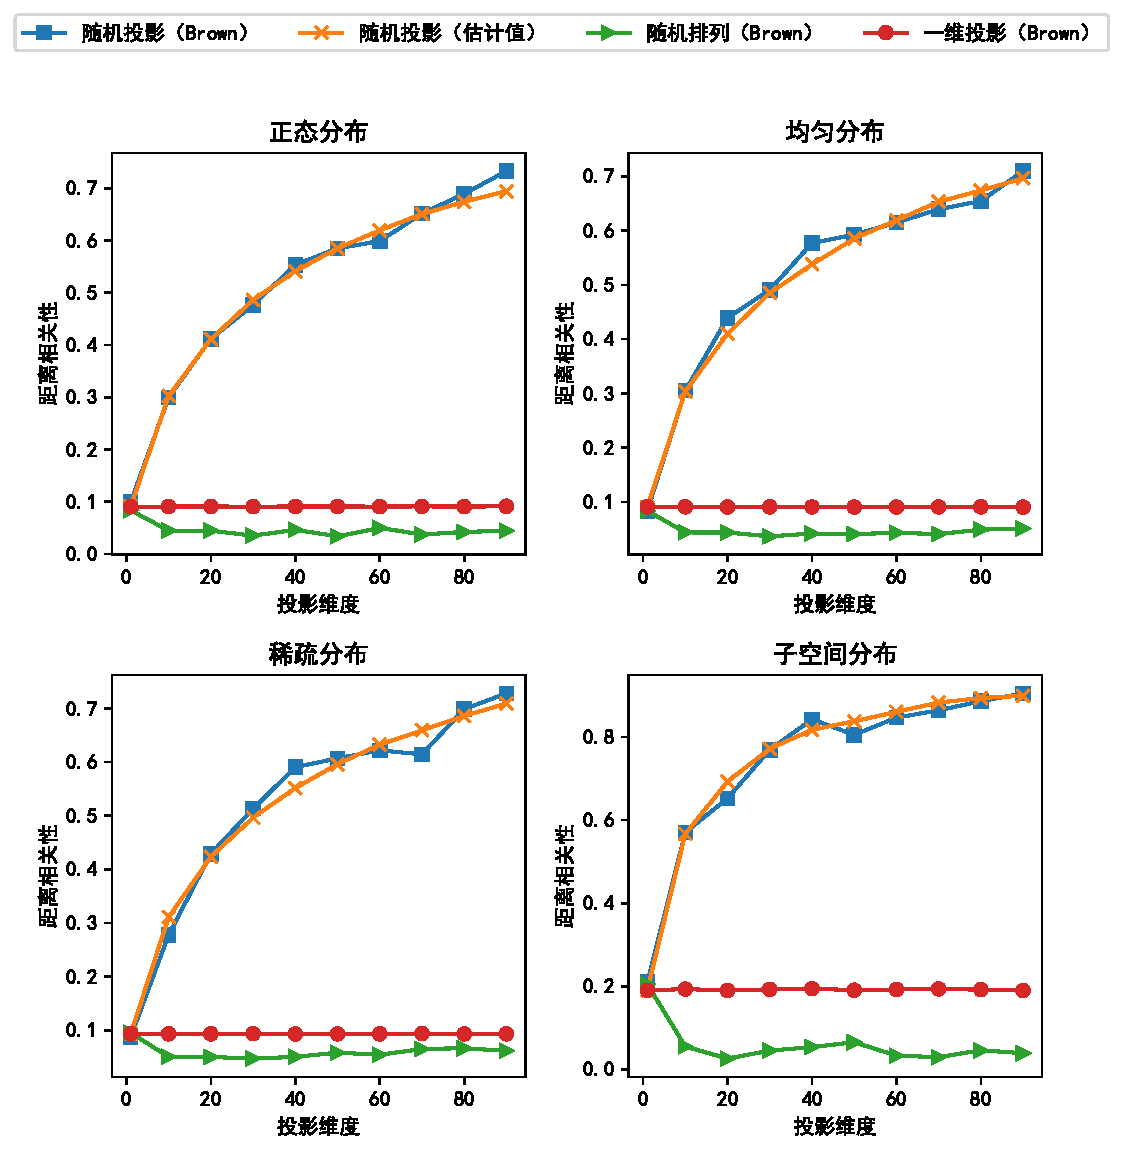
\includegraphics[width=\linewidth]{Z_Resources/ss-perm_dcor-estimation}
    \caption{各种数据分布下随机投影和随机排列的距离相关性}
    \label{fig:ss-perm:dcor-estimation}
\end{figure}


对于每个分布,我们采样1万个点(记作$X$),然后使用高斯分布的矩阵投影得到$Y = WX$,最后对投影后的向量进行随机排列得到$\pi[Y]$。
%
我们采用文献~\cite{szekely2009brownian_dcor}中的基于布朗运动(Brownian Motion)的方法对距离相关性进行数值计算(标记为“Brown”),同时也使用\autoref{eq:ss-perm:linear-dcor-estimation}对随机投影的距离相关性进行估算(标记为“估计值”),并一同呈现在\autoref{fig:ss-perm:dcor-estimation}中。
%


上述数值模拟表明,随机投影后的数据与原始数据具有较大的距离相关性,且投影后的维度越高,距离相关性越大。
%
而本文在投影后的数据上进一步采用随机排列,极大减少了距离相关性。
且无论投影维度变化,其距离相关性一直小于一维投影的距离相关性,验证了本节的理论分析结论。